\chapter{ECUACIONES DE EULER Y APLICACIÓN DEL ESQUEMA DE ROE}

En este capítulo se explican y derivan las ecuaciones de Euler utilizando las variables generales (presión, densidad y velocidad) y se introducen las variables conservadas. Se explican las ligaduras adicionales involucradas para que las ecuaciones de Euler sean aplicadas a un gas ideal poliatómico.

Se describe el esquema de Roe implementado en la solución de las ecuaciones de Euler para un gas ideal poliatómico así como las demás especificaciones requeridas por el método de volúmenes finitos. Se explica la implementación del método numérico en \texttt{C++}. Se muestran los resultados obtenidos para un problema de condiciones iniciales específicas.
\section{Ecuaciones de Euler}
Las ecuaciones fundamentales de la dinámica de fluidos se basan en las siguientes leyes de conservación universales:
\begin{itemize}
	\item Conservación de la masa
	\item Conservación del momentum
	\item Conservación de la energía.
\end{itemize}
La ecuación de conservación de la masa, que se derivó en la sección \ref{sec:derivacion-continuidad}, consiste en aplicar la ecuación de continuidad para un fluido con cierta densidad. La ley de conservación del momentum resulta al aplicar la Segunda Ley de Newton en un fluido. Por último, la ley de conservación de la energía es equivalente a la aplicación de la Primera Ley de la Termodinámica. Además de las tres ecuaciones de conservación, es necesario establecer una relación entre las variables físicas del fluido, de tal manera que el sistema de ecuaciones sea resoluble \cite{heattransfer}. En el caso de un gas ideal, la ecuación adicional que relaciona las variables densidad $\rho$, presión $p$ y temperatura $T$, es la ecuación de estado. 
\subsection{Derivación de las ecuaciones}
%\subsubsection{Ecuación de continuidad}
La ecuación de continuidad, derivada en la sección \ref{sec:derivacion-continuidad} tiene la siguiente forma
\begin{equation}
	\rho_{t} + (\rho v)_{x} = 0.
	\label{eq:continuidad-euler}
\end{equation}
Ya que el flujo asociado a esta ecuación de conservación es $\rho v$, se puede interpretar que, generalmente, para cualquier cantidad física $z$ que sufra advección, su flujo estará dado por el producto de la cantidad por la velocidad de advección, i.e., $f=zv$. 

A partir del último razonamiento, el flujo asociado a la advección de momentum $\rho v$, tiene una contribución al flujo dada por $(\rho v) \cdot v = \rho v^2$. Sin embargo, además de la advección que sufre el momentum, deben considerarse las fuerzas que actúan en el fluido para expresar el flujo total del momentum. En este texto no se considerarán fuerzas externas, por lo que únicamente habría que tomar en cuenta la fuerza interna del fluido, que está dada por el gradiente de \textbf{presión}, $p_x$ \cite{LeVeque}. De esta manera, se consigue la ecuación de conservación del momentum:
\begin{equation}
	(\rho v)_t + (\rho v^{2} + p)_{x} = 0.
	\label{eq:momentum-euler}
\end{equation}

Para derivar la conservación de energía, se debe considerar que ésta se compone por un término cinético y uno correspondiente a la energía interna del fluido. Sea $E$ la densidad de energía total de un fluido. Entonces, se tiene que:
\begin{equation}
	E = \frac{1}{2} v^{2} + e,
	\label{eq:energia}
\end{equation}
donde el término $\frac{1}{2} v^{2}$ corresponde a la densidad de energía cinética por unidad de masa y $e$ es la \textbf{energía interna} por unidad de masa del fluido, que también suele denominarse como energía interna específica. La energía interna depende de los grados de libertad internos de las moléculas de los gases, considerando energía de rotación, cinética, de vibración y otras formas más complejas de energía. Las ecuaciones de Euler suponen que la ecuación de estado provee una expresión para la energía interna específica tal que ésta depende de la presión y la densidad del fluido únicamente
\begin{equation}
	e = e(p, \rho).
\end{equation}
De igual manera que con el momentum, la energía total se ve afectada por la advección del flujo del fluido. Dado que no se consideran fuerzas externas que afecten al sistema, únicamente la presión del fluido hace trabajo y es proporcional al gradiente de $vp$. Entonces la ecuación de conservación de la energía se reduce a:
\begin{equation}
	(\rho E)_{t} + [v(\rho E + p)]_{x} = 0.
	\label{eq:energia-euler}
\end{equation}
Haciendo notar que $\rho E$ corresponde a la energía total del gas.

Las ecuaciones de Euler, (\ref{eq:continuidad-euler}), (\ref{eq:momentum-euler}) y (\ref{eq:energia-euler}) se pueden escribir en forma vectorial, obteniendo:
\begin{equation}
	\begin{bmatrix}
		\rho \\
		\rho v \\
		\rho E
	\end{bmatrix}_{t}
+
	\begin{bmatrix}
		\rho v \\
		\rho v^{2}+p \\
		v(\rho E + p)
	\end{bmatrix}_{x}
= 0,
\label{eq:euler-eqs-1}
\end{equation}
cuya forma coincide con la presentada en (\ref{eq:conservacion}). Cabe mencionar que en este texto se considerarán problemas unidimensionales solamente.

%Para escribir el sistema (\ref{eq:euler-eqs-1}) de la forma (\ref{eq:conservacion-jacobiana}) 

\subsection{Ecuación de estado para un gas politrópico}
Para completar el sistema de ecuaciones de Euler, es necesario definir la ecuación de estado que relacione la energía con las variables físicas de presión y  densidad. El desarrollo de la ecuación de estado para un gas ideal sigue de cerca la sección \textit{Ideal Gas} del capítulo \textit{Some Linear Systems} en \cite{LeVeque}.

La energía interna de un gas ideal es únicamente dependiente de la temperatura,
\begin{equation}
	e = e(T).
\end{equation}
Mientras que la temperatura se relaciona con la presión y densidad a través de la ley del gas ideal, que define al mismo. Esta es:
\begin{equation}
	p = \mathcal{R}\rho T
	\label{eq:ideal-gas-law}
\end{equation}
donde $\mathcal{R}$ es la constante específica de los gases, que se define como el cociente entre la constante de Boltzmann $k_B$ y  la masa de cada molécula del gas $m$ \cite{blundell}. Por otro lado, la energía interna específica es proporcional a la temperatura,
\begin{equation}
	e = c_{v}T
	\label{eq:energia-interna-1}
\end{equation}
donde $c_{v}$ es la capacidad calorífica específica a volumen constante. Los gases que cumplen con esta propiedad se conocen como gases \textbf{politrópicos}. Entonces, si se cambiase la temperatura de un gas en una cantidad infinitesimal $\dd{T}$, manteniendo el volumen constante, se obtendría
\begin{equation}
	\dd{e} = c_{v} \dd{T}
\end{equation}
como cambio infinitesimal de energía interna específica. En cambio, si se permite que el gas se expanda pero manteniendo ahora la presión constante, se obtendría una expresión para el cambio de energía considerando al trabajo, $\dd{W} = -p\dd{V}$, realizado sobre el gas, esto es
\begin{equation}
	m\dd{e} = \dd{W} + \dbar Q
\end{equation}
\begin{equation}
	m\dd{e} = -p\dd{V} + \dbar Q
\end{equation}
\begin{equation}
	\dd{e} = -\frac{p}{m}\dd{V} + c_{p}\dd{T}
\end{equation}
y puesto que al usar $\rho = \frac{m}{V}$, se obtiene que $\dd{V} = m\dd(\frac{1}{\rho})$, entonces:
\begin{equation}
	\dd{e} = -p\dd(\frac{1}{\rho}) + c_{p}\dd{T}
\end{equation}
\begin{equation}
	\dd(e + \frac{p}{\rho}) = c_{p}\dd{T},
	\label{eq:entalpia-temp-dif}
\end{equation}
donde $c_p$ es la capacidad calorífica específica del gas a presión constante. A partir del anterior resultado se define la \textbf{entalpía} interna $\mathrm{h}_i$:
\begin{equation}
	\mathrm{h}_i \equiv e + \frac{p}{\rho},
	\label{eq:entalpia-1}
\end{equation}
mientras que la entalpía total $\mathrm{h}$ \footnote{No confundir con $h$ definida en \ref{eq:def-h} como el tamaño de cada celda del dominio.} es:
\begin{equation}
	\mathrm{h} = E + \frac{p}{\rho}.
	\label{eq:entalpia-total}
\end{equation}
Para un gas politrópico se considera a $c_p$ como constante, por lo que integrando la ecuación (\ref{eq:entalpia-temp-dif}) se obtiene otra expresión para la entalpía interna,
\begin{equation}
	\mathrm{h}_i = c_p T.
	\label{eq:entalpia-2}
\end{equation}
Por otro lado, de acuerdo a la ley del gas ideal, se tiene la siguiente relación
\begin{equation}
	c_p - c_v = \mathcal{R}.
	\label{eq:diferencia-capacidades}
\end{equation}
Para continuar con la derivación, es conveniente definir el \textbf{coeficiente de dilatación adiabática} $\gamma$ como:
\begin{equation}
	\gamma \equiv \frac{c_p}{c_v}.
	\label{eq:gamma-1}
\end{equation}
Dicha cantidad está estrechamente relacionada con el número de grados de libertad internos del gas, que depende de la naturaleza del mismo. Según el teorema de equipartición de la energía, el promedio de energía involucrada en cada grado de libertad es el mismo. Específicamente, cada grado de libertad aporta una cantidad promedio de energía por molécula de $\frac{1}{2}k_B T$. De tal manera que si existen ${\alpha}$ grados de libertad internos en un gas que tiene $n$ moléculas por unidad de masa, se obtiene una expresión para la energía interna específica
\begin{equation}
	e = \frac{\alpha}{2}n k_B T
\end{equation}
o bien, 
\begin{equation}
	e = \frac{\alpha}{2}\mathcal{R} T.
	\label{eq:energia-interna-2}
\end{equation}
Comparando con (\ref{eq:energia-interna-1}) se obtiene
\begin{equation}
	c_v = \frac{\alpha}{2}\mathcal{R},
\end{equation}
sustituyendo en (\ref{eq:diferencia-capacidades}),
\begin{equation}
	c_p = \left(1+\frac{\alpha}{2}\right)\mathcal{R}.
\end{equation}
Y al aplicar la definición de $\gamma$ en (\ref{eq:gamma-1}) se obtiene la expresión
\begin{equation}
	\gamma = \frac{\alpha + 2}{\alpha},
\end{equation}
que, como se expuso previamente, relaciona el número de grados de libertad con el coeficiente de dilatación adiabática. Por ejemplo, para gases monoatómicos se consideran únicamente tres grados de libertad, correspondientes al movimiento traslacional en tres dimensiones, por lo que $\alpha = 3$ y $\gamma = 5/3$. En gases diatómicos (como el aire, compuesto por $\mathrm{H}_2$ y $\mathrm{N}_2$ principalmente) se agregan dos grados libertad correspondientes a dos ejes de rotación posibles para cada molécula, de tal manera que $\alpha = 5$ y $\gamma = 7/5 = 1.4$.

Por último, se escribe la ecuación de estado del gas ideal para la energía utilizando  (\ref{eq:ideal-gas-law}),
\begin{equation}
	e = c_v T = \frac{c_v}{\mathcal{R}}\cdot\frac{p}{\rho}
\end{equation}
\begin{equation}
	e = \frac{p}{(\gamma - 1) \rho}.
\end{equation}
De tal manera que la energía total del gas ($\rho E$) queda como
\begin{equation}
	 \rho E = \frac{1}{2}\rho v^{2} + \frac{p}{\gamma - 1}.
	 \label{eq:energia-total}
\end{equation}
\section{Aplicación del esquema de Roe}
Para aplicar el esquema de Roe en la expresión del método de volúmenes finitos, dada por 
\begin{equation}
	U_{i}^{n+1}-U_{i}^{n} = 
	\frac{k}{h}\left[ F(U_{i-1}^n, U_i^n) - F(U_{i}^n, U_{i+1}^n) \right],
	\label{eq:metodo-vol-finitos-3}
\end{equation}
 es necesario definir el flujo entre cada interfaz, $F_{i\pm \frac{1}{2}}$. La expresión de dicho flujo, en su forma simple, se detalló en (\ref{eq:roe-flux}). Mientras que la versión del flujo en conjunto con la corrección de entropía es (\ref{eq:flux-HH-fix}). Por tanto, el siguiente paso es construir el flujo de Roe de acuerdo a las aproximaciones correspondientes.
\subsection{Variables conservadas y propiedades de $\mathbf{A(\mathbf{U})}$}
Para implementar el método de volúmenes finitos junto al esquema de Roe en la solución numérica de las ecuaciones de Euler es necesario identificar las \textbf{variables conservadas} involucradas en la definición de un sistema general de conservación, definido en (\ref{eq:conserv-deriv-short}). Comparando esta expresión con el sistema (\ref{eq:euler-eqs-1}) se obtiene:
\begin{equation}
	\mathbf{U} = 
	\begin{bmatrix}
		\mathbf{u}_1 \\
		\mathbf{u}_2 \\
		\mathbf{u}_3
	\end{bmatrix} \equiv
	\begin{bmatrix}
		\rho \\
		\rho v \\
		\rho E
	\end{bmatrix}
\end{equation}
\begin{equation}
	\mathbf{F} = 
	\begin{bmatrix}
		\mathbf{f}_1 \\
		\mathbf{f}_2 \\
		\mathbf{f}_3
	\end{bmatrix} \equiv
	\begin{bmatrix}
		\rho v \\
		\rho v^2 + p \\
		v(\rho E + p)
	\end{bmatrix}.
\label{eq:flujo-euler-exacto}
\end{equation}
Por tanto, se define a $\mathbf{u}_i$ como la i-ésima variable conservada cuyo  flujo correspondiente es $\mathbf{f}_i$. 

Por otro lado, el esquema de Roe depende de los autovalores y autovectores de la matriz jacobiana $\mathbf{A(\mathbf{U})}$ definida en (\ref{eq:conservacion-jacobiana}). Aplicando la definición (\ref{eq:jacobiana-A-definicion}) mientras se toma en cuenta la ecuación de estado para la energía (\ref{eq:ideal-gas-law}), se obtiene una expresión para esta matriz:
\begin{equation}
	\mathbf{A(\mathbf{U})} =
	\begin{bmatrix}
		0 & 1 & 0 \\
		\frac{1}{2}(\gamma - 3)v^2 & (3  - \gamma) v & (\gamma - 1) \\
		\frac{1}{2}(\gamma - 1)v^3 - v(\rho E+p)/\rho & (\rho E+p)/\rho-(\gamma - 1)v^2 & \gamma v \\
	\end{bmatrix}.
\end{equation}
Seguidamente, se deben calcular los autovalores y autovectores de esta matriz. Siguiendo la notación de los últimos capítulos, al autovalor $\lambda_i$ le corresponde el autovector $\mathbf{r}_i$, y estos son:
\begin{equation}
	\lambda_1 = v-c, \hspace{4mm}
	\lambda_2 = c, \hspace{4mm}
	\lambda_3 = v+c,
\end{equation}
\begin{equation}
	\mathbf{r}_1 = 
	\begin{bmatrix}
		1 \\
		v-c \\
		\mathrm{h}-vc
	\end{bmatrix},\hspace{4mm}
	\mathbf{r}_2 = 
	\begin{bmatrix}
		1 \\
		v \\
		\frac{1}{2}v^{2}
	\end{bmatrix},\hspace{4mm}
	\mathbf{r}_3 = 
	\begin{bmatrix}
		1 \\
		v+c \\
		\mathrm{h}+vc
	\end{bmatrix}.
\end{equation}
donde $c$ es la velocidad del sonido, dada por:
\begin{equation}
	c = \sqrt{\frac{\gamma p}{\rho}},
\end{equation}
mientras $\mathrm{h}$ es la entalpía total definida en (\ref{eq:entalpia-total}), o bien, equivalentemente:
\begin{equation}
	\mathrm{h} = \frac{1}{2}v^2 + \left(\frac{\gamma}{\gamma - 1}\right)\frac{p}{\rho}.
\end{equation}
Por lo tanto, es posible escribir la velocidad del sonido en términos de la entalpía y la velocidad:
\begin{equation}
	c^2 = (\gamma - 1)\left[\mathrm{h} - \tfrac{1}{2}v^{2}\right].
\end{equation}
\subsection{Valores promediados de Roe}
Retornando a la expresión para el flujo numérico simple de Roe,
\begin{equation}
	F(\mathbf{U}_L, \mathbf{U}_R) = \frac{1}{2}\left(\mathbf{F}(\mathbf{U}_L) +\mathbf{F}(\mathbf{U}_R)\right) - 
	\frac{1}{2}\sum_{p=1}^{m}|\hat{\lambda}_{p}|\alpha_{p}\mathbf{\hat{r}}_{p},
	\label{eq:roe-flux-2}
\end{equation}
se destaca que es necesario encontrar los autovalores $\hat{\lambda}_i$ y autovectores $\hat{r}_i$ correspondientes a la matriz aproximada $\mathbf{\hat{A}}$. Roe \cite{roe81} propuso expresiones, basadas en promedios específicos de los valores adyacentes, para los mencionados autovectores y autovalores de la matriz aproximada y junto a Pike demostraron que son los únicos promedios que satisfacen las condiciones necesarias impuestas al flujo numérico del esquema de Roe \cite{roe86}. Los autovalores y autovectores de Roe son:
\begin{equation}
	\hat{\lambda}_1 = \tilde{v}-\tilde{c}, \hspace{4mm}
	\hat{\lambda}_2 = \tilde{c}, \hspace{4mm}
	\hat{\lambda}_3 = \tilde{v}+\tilde{c},
\end{equation}
\begin{equation}
	\mathbf{\hat{r}}_1 = 
	\begin{bmatrix}
		1 \\
		\tilde{v}-\tilde{c} \\
		\tilde{\mathrm{h}}-\tilde{v}\tilde{c}
	\end{bmatrix},\hspace{4mm}
	\mathbf{\hat{r}}_2 = 
	\begin{bmatrix}
		1 \\
		\tilde{v} \\
		\frac{1}{2}\tilde{v}^{2}
	\end{bmatrix},\hspace{4mm}
	\mathbf{\hat{r}}_3 = 
	\begin{bmatrix}
		1 \\
		\tilde{v}+\tilde{c} \\
		\tilde{\mathrm{h}}+\tilde{v}\tilde{c}
	\end{bmatrix}.
\end{equation}
 Mientras que los coeficientes de las características $\alpha_{i}$ están dados por:
 \begin{equation}
 	\alpha_1 = \frac{1}{2\tilde{c}^{2}}[\Delta p - \tilde{\rho}\tilde{c}\Delta v], \hspace{4mm}
 	\alpha_2 = \frac{1}{\tilde{c}^{2}}\left[\tilde{c}^{2}\Delta\rho - \Delta p\right], \hspace{4mm}
 	\alpha_3 = \frac{1}{2\tilde{c}^{2}}[\Delta p + \tilde{\rho}\tilde{c}\Delta v],
 \end{equation}
con
\begin{equation}
	\tilde{\rho} = \sqrt{\rho_L \rho_R}
	\label{eq:rho-prom}
\end{equation}
\begin{equation}
	\tilde{v} = \frac{\sqrt{\rho_{L}}\cdot v_L + \sqrt{\rho_{R}}\cdot v_R}{\sqrt{\rho_{L}} + \sqrt{\rho_{R}}}
\end{equation}
\begin{equation}
	\tilde{\mathrm{h}} = \frac{\sqrt{\rho_{L}}\cdot \mathrm{h}_L + \sqrt{\rho_{R}}\cdot \mathrm{h}_R}{\sqrt{\rho_{L}} + \sqrt{\rho_{R}}}
\end{equation}
\begin{equation}
	\tilde{c}^{2} = (\gamma - 1)[\tilde{h} - \tfrac{1}{2}\tilde{v}^2]
	\label{eq:c-prom}
\end{equation}
donde $\Delta u = u_R - u_L$, para cualquier variable $u$, siendo $u_R$ y $u_L$ el valor de la variable a la derecha e izquierda de la interfaz en donde se calcula el flujo, respectivamente.
\section{Características básicas de la simulación}
Para resolver las ecuaciones de Euler es necesario especificar algunas características del medio y  del espacio en el que toman lugar las simulaciones a presentar en este texto. 
\subsection{Dimensiones}
\label{sec:dimensiones}
Las ecuaciones de Euler serán resueltas en una dimensión espacial, que se puede interpretar como la evolución temporal de un gas dentro de un tubo. Naturalmente, un tubo no es exactamente un objeto unidimensional (un objeto unidimensional es una idealización) pero se aproximará como tal para efectuar la simulación. Este dominio posee una longitud de $10\unit{\meter}$, de tal manera que definiendo los parámetros de la sección \ref{sec:discretizacion-del-dominio}, se tiene:
\begin{equation}
	a = 0 \unit{\meter},
\end{equation}
\begin{equation}
	b = 10 \unit{\meter}.
\end{equation}
Es natural entonces definir una variable para el largo del dominio, $L\equiv b-a$. Mientras que el número de celdas $N$ a utilizar será:
\begin{equation}
	N = 500.
\end{equation}
De tal forma que el tamaño de cada celda está dado por:
\begin{equation}
	h = \frac{10\unit{\meter}}{500} = 0.02 \unit{\meter}.
\end{equation}
El tiempo total por defecto será de $4\unit{\second}$, y se producirá la solución para un número determinado de instantes temporales en total, que generalmente no coincidirá con el número de instantes temporales calculados. Esto se hace para optimizar el tiempo de cómputo. Por esta razón, el tamaño de paso temporal $k$ puede estar sujeto a cambios dependiendo de la simulación, ya que en caso no se cumpla la condición de estabilidad (\ref{eq:cond-estabilidad}) deberán recalibrarse los parámetros temporales.

A excepción de los resultados mostrados en el capítulo \ref{cap:5}, se tomará el coeficiente de dilatación adiabática como el valor aproximado que posee el aire, $\gamma = 1.4$ \cite{LeVeque}.

\subsection{Condiciones iniciales}
Se experimentará con tres distintos conjuntos de condiciones iniciales para las ecuaciones de Euler. 

\subsubsection{Primer conjunto}
\label{sec:gaussiana41}
Este conjunto corresponde a una solución trivial. Las condiciones iniciales de las variables físicas son las siguientes
\begin{align}
	&\rho(x,0) =  \left(1.0+\exp[-(x-\tfrac{L}{2})^{2}]\right)\hspace{1mm}\unit{\kilogram\per\meter^{3}} \\
	&v(x,0) = 1.0 \hspace{1mm}\unit{\meter\per\second} \\
	&p(x,0) = 0.5 \hspace{1mm}\unit{\pascal}
\end{align}
Notando que tanto la velocidad como la presión son constantes, se espera que el perfil gaussiano definido para la densidad se traslade a velocidad constante sobre el eje $x$. Esto se deriva del hecho de que la ecuación de continuidad \eqref{eq:continuidad-euler} se reduce a una ecuación de advección lineal en este caso.

Los siguientes conjuntos de condiciones iniciales corresponden a funciones definidas por partes. Las variables tendrán un valor constante que depende de la mitad del dominio en donde se valúen. Se adoptará la siguiente notación para escribir de manera compacta las condiciones iniciales:
\begin{equation}
	\mathbf{V}(x,0) = 
	\begin{cases}
		\mathbf{V}_{L} & \text{ si } x \leq L/2\\
		\mathbf{V}_{R} & \text{ si } x > L/2,
	\end{cases}
\end{equation}
donde
\begin{equation}
\mathbf{V}(x,t) = 
	\begin{bmatrix}
		\rho \\
		v \\
		P
	\end{bmatrix},
\end{equation}
es el vector de variables físicas independientes.

\subsubsection{Segundo conjunto}
\label{sec:sod_con_entropy148}
Este conjunto de condiciones iniciales se denomina Test de Sod \cite{thesis-euler-godunov}. Consiste en los siguientes valores para las variables físicas independientes \footnote{Se omiten las dimensiones de las variables para mantener la legibilidad del texto, sin embargo, todas las unidades utilizadas corresponden a las del Sistema Internacional.}

\begin{equation}
\mathbf{V}_L = 
	\begin{bmatrix}
		3.0\\
		0.0\\
		3.0
	\end{bmatrix},\hspace{4mm}
\mathbf{V}_R = 
	\begin{bmatrix}
		1.0\\
		0.0\\
		1.0
	\end{bmatrix}.
\end{equation}
En este conjunto de condiciones iniciales se destaca la diferencia de presión en cada mitad del dominio, así como de la densidad, que va de mayor a menor cantidad. La velocidad inicial del gas es nula.

\subsubsection{Tercer conjunto}
\label{sec:leveque_sin_entropy714}
El siguiente conjunto de condiciones iniciales fue propuesto por LeVeque para evaluar el funcionamiento del esquema numérico utilizado cuando se presentan ondas de rarefacción transónica \cite{pelanti}. Es similar al test de Sod, pero con la diferencia que la velocidad inicial del gas no es nula. Los valores iniciales son:
\begin{equation}
	\mathbf{V}_L = 
	\begin{bmatrix}
		3.0\\
		0.9\\
		3.0
	\end{bmatrix},\hspace{4mm}
	\mathbf{V}_R = 
	\begin{bmatrix}
		1.0\\
		0.9\\
		1.0
	\end{bmatrix}.
\end{equation}
\subsection{Condiciones de frontera}
Previo a poder aplicar el método de volúmenes finitos (MVF) junto al esquema de Roe, es necesario especificar las condiciones de frontera en el dominio espacial.
De acuerdo a la expresión (\ref{eq:metodo-vol-finitos-3}), generalmente el MVF se aplica sobre un dominio dividido en $N$ celdas, de manera que el índice $i$ se recorre de $1$ a $N$. Por lo tanto, es necesario definir los valores de la frontera, siendo estos $U_{0}^{n}$ y $U_{N+1}^{n}$, para que los flujos $F_{\frac{1}{2}}$ y $F_{N+\frac{1}{2}}$ estén bien definidos y correspondan a flujos físicamente consistentes.
\subsubsection{Condiciones transmisivas}
Si se asume que el gas se encuentra dentro de un tubo con las paredes extremas abiertas, se pueden considerar condiciones que permitan la transmisión del medio al exterior \cite{thesis-euler-godunov}. Las condiciones de frontera transmisivas se puede conseguir con las siguientes igualdades:
\begin{align}
	\rho_{0}^{n} = \rho_{1}^{n}, \hspace{4mm}&
	\rho_{N+1}^{n} = \rho_{N}^{n} \\
	v_{0}^{n} = v_{1}^{n}, \hspace{4mm}&
	v_{N+1}^{n} = v_{N}^{n} \\
	p_{0}^{n} = p_{1}^{n}, \hspace{4mm}&
	p_{N+1}^{n} = p_{N}^{n}.
\end{align}
\section{Código implementado}
\lstset{inputencoding=utf8/latin1}
Como fue comentado previamente, la solución numérica de las ecuaciones de Euler se implementó en un programa de \texttt{C++}. El código fuente completo de la simulación se encuentra disponible en \url{https://github.com/highchen147/tesis/blob/main/euler1D/euler1D.cpp}.

\subsection{Librerías y paquetes utilizados}
Se utilizaron las siguientes librerías en el desarrollo del programa integrador:
\lstinputlisting[title = Librerías,
language=C++,
firstline=1,
lastline=12,
keywordstyle=\color{blue}]{../euler1D/code_en_TDG/preambulo.cpp}

En el paquete con nombre \texttt{funciones.hpp} se definió una función por partes, con nombre \texttt{step\_neg}, para aplicar las condiciones iniciales de forma práctica.

\lstinputlisting[
caption={Función \texttt{step\_neg}},
label=cod:step-neg,
language=C++,
firstline=13,
lastline=24,
keywordstyle=\color{blue}
]{../euler1D/code_en_TDG/preambulo.cpp}

\subsection{Definición de parámetros principales}
Se definió el coeficiente de dilatación adiabática como una variable global, esto con el fin de evitar escribir muchas funciones en donde dicho coeficiente fuera un parámetro de las mismas y así contar con una variable constante y segura para toda la simulación.

\lstinputlisting[
caption = {Definición de $\gamma$},
%label
language=C++,
firstline=1,
lastline=1,
keywordstyle=\color{blue}]{../euler1D/code_en_TDG/parametros.cpp}

Se definieron seis parámetros temporales en la función \texttt{int main()} del programa:
\lstinputlisting[
caption = {Parámetros temporales},
language=C++,
firstline=3,
lastline=10,
keywordstyle=\color{blue}]{../euler1D/code_en_TDG/parametros.cpp}

Los parámetros \texttt{t\_total}, \texttt{dt} y \texttt{num\_outs} son modificables de acuerdo a lo necesario para conseguir una simulación satisfactoria. \texttt{t\_total} es el tiempo total de la simulación, mientras que \texttt{dt} es el tamaño de paso temporal que fue definido en el capítulo \ref{cap:2} como $k$. El parámetro \texttt{Niter} se define como el número de iteraciones necesarias temporales para conseguir una simulación que dure lo preestablecido y coincida con el tamaño de paso \texttt{dt}; además, se usa la función \texttt{floor()} para garantizar un número entero de iteraciones. 

La variable \texttt{num\_outs} almacena el número de soluciones producidas para estados temporales determinados, es decir, se imprimen los datos de las funciones calculadas para \texttt{num\_outs} instantes temporales, que no necesariamente coincidirá con el número de iteraciones. Luego se define \texttt{out\_cada}, que calcula cada cuántas iteraciones se deberán imprimir los datos. Por último, la variable \texttt{tiempo} almacena el tiempo real de la simulación.

Los parámetros espaciales, que fueron descritos en la sección \ref{sec:dimensiones} se definieron de la siguiente manera en el código:
\lstinputlisting[
caption = {Parámetros espaciales},
language=C++,
firstline=12,
lastline=14,
keywordstyle=\color{blue}]{../euler1D/code_en_TDG/parametros.cpp}

Por último, se definió una variable de tipo booleana, para activar o desactivar la corrección de entropía. En otras palabras, esta variable decide si se usa el flujo simple de Roe (\ref{eq:roe-flux}) o el flujo modificado para corregir el caso de entropía sónica (\ref{eq:flux-HH-fix}).
\lstinputlisting[
caption = {Corrección de entropía},
language=C++,
firstline=17,
lastline=17,
keywordstyle=\color{blue}]{../euler1D/code_en_TDG/parametros.cpp}
\subsection{Objetos definidos}
Las soluciones numéricas son aproximaciones en forma discreta, por lo que para construir las funciones de magnitudes físicas en el programa, se definieron punteros a arreglos unidimensionales, con un tamaño que coincidiera con el número de celdas definido para la simulación \footnote{A diferencia del resto del texto, se definió a la velocidad del gas como \texttt{u}.}.
\lstinputlisting[
caption = {Arreglos de variables físicas},
language=C++,
firstline=2,
lastline=11,
keywordstyle=\color{blue}]{../euler1D/code_en_TDG/objetos.cpp}

Las variables \texttt{rho}, \texttt{u} y \texttt{p} corresponden a las funciones de densidad, velocidad y presión valuadas en el instante temporal $n$, respectivamente. Las variables cuyo nombre lleva el sufijo \texttt{\_nueva} corresponden a la cantidad valuada en el instante temporal siguiente $n+1$, i.e,
\begin{equation}
	\rho_{i}^{n} \leftrightarrow \texttt{rho[i]}
\end{equation}
\begin{equation}
	\rho_{i}^{n+1} \leftrightarrow \texttt{rho\_nueva[i]}.
\end{equation}

También se definieron arreglos para las componentes del vector $\mathbf{{U}}$, siendo \texttt{ui} la iésima componente de $\mathbf{{U}}$.
\lstinputlisting[
caption = {Componentes vectoriales},
language=C++,
firstline=12,
lastline=15,
keywordstyle=\color{blue}]{../euler1D/code_en_TDG/objetos.cpp}

El vector en cuestión fue implementado como un objeto de la clase \texttt{vector} de tipo \texttt{double} con dimensión 3. El uso de objetos de dicha clase fue con el objetivo de utilizar la sobrecarga de los operadores básicos (\texttt{+}, \texttt{-}, \texttt{*}) para realizar operaciones entre los vectores prácticamente. La definición de la acción de los operadores se omitirá en este texto, ya que su funcionamiento e implementación son triviales. 
\lstinputlisting[
caption = {Componentes vectoriales},
label=cod:definicion-U,
language=C++,
firstline=23,
lastline=24,
keywordstyle=\color{blue}]{../euler1D/code_en_TDG/objetos.cpp}

El dominio se dividió en celdas, cuya ubicación en el espacio se almacenó en un puntero.
\lstinputlisting[
caption = {Arreglo de celdas},
language=C++,
firstline=20,
lastline=21,
keywordstyle=\color{blue}]{../euler1D/code_en_TDG/objetos.cpp}
\subsection{Inicialización de arreglos}
Para inicializar cada arreglo previamente definido se utilizaron ciclos iterativos.
\lstinputlisting[
caption = {Inicialización de variables},
language=C++,
firstline=2,
lastline=16,
keywordstyle=\color{blue}]{../euler1D/code_en_TDG/inicializacion.cpp}

Las funciones \texttt{rho\_inicial}, \texttt{p\_inicial}, \texttt{u\_inicial} son variaciones de la función por partes, definida en el código (\ref{cod:step-neg}), que dependen de la condición inicial por aplicar. Por ejemplo, la condición de  la sección \ref{sec:leveque_sin_entropy714} para la velocidad, se aplica de la siguiente manera:
\lstinputlisting[
caption = {Condición inicial para la velocidad},
language=C++,
firstline=18,
lastline=21,
keywordstyle=\color{blue}]{../euler1D/code_en_TDG/inicializacion.cpp}

La inicialización de las componentes de $\mathbf{{U}}$ se realizó con una función de tipo \texttt{void} para facilitar la escritura en el código del cálculo de las componentes del mismo vector.
\lstinputlisting[
caption = {Cálcuo de las componentes del vector de cantidades conservadas},
language=C++,
firstline=23,
lastline=48,
keywordstyle=\color{blue}]{../euler1D/code_en_TDG/inicializacion.cpp}
Se puede apreciar que los cálculos de las componentes de $\mathbf{{U}}$ coinciden con (\ref{eq:euler-eqs-1}) tomando en cuenta la definición de la energía (\ref{eq:energia-total}).
\subsection{Funciones auxiliares del esquema de Roe}
Previo a la descripción del ciclo iterativo de la integración numérica, se muestra la construcción de las funciones que completan la implementación en el programa de la expresión (\ref{eq:metodo-vol-finitos-2}).

La función \texttt{flujo\_euler} calcula el flujo exacto del sistema de Euler. En otras palabras, es la implementación directa de $\mathbf{{F}}$, definido en (\ref{eq:flujo-euler-exacto}).
\lstinputlisting[
caption = {Definición de la función que calcula el flujo del sistema de Euler},
language=C++,
firstline=1,
lastline=18,
keywordstyle=\color{blue}]{../euler1D/code_en_TDG/flujos.cpp}
Cabe destacar que el flujo de Euler se implementa como un objeto de la clase \texttt{vector}, de la misma manera que se define \texttt{U}, como se expuso en el código (\ref{cod:definicion-U}).

Evidentemente, el flujo exacto de Euler no es igual al flujo numérico de Roe, sino que el último depende del primero. El flujo de Roe se construyó  por partes en el programa. A continuación se muestra la implementación de $F(\mathbf{{U}}_L, \mathbf{{U}}_R)$, correspondiente a la ecuación (\ref{eq:roe-flux}).
\lstinputlisting[
caption = {Definición de la función que devuelve el flujo numérico},
language=C++,
firstline=20,
lastline=65,
keywordstyle=\color{blue}]{../euler1D/code_en_TDG/flujos.cpp}
Esta función retorna un objeto de la clase \texttt{vector}. La función \texttt{suma\_p} corresponde al cálculo de la suma $\sum_{p=1}^{m}|\hat{\lambda}_{p}|\alpha_{p}\mathbf{\hat{r}}_{p}$. Por otro lado, la función \texttt{suma\_p\_fix} corresponde a la modificación de la anterior implementando la corrección de entropía, es decir, calcula la suma $\sum_{p=1}^{m}H(\hat{\lambda}_{p})\alpha_{p}\mathbf{\hat{r}}_{p}$, definida en la ecuación (\ref{eq:flux-HH-fix}). A continuación se muestra el código implementado de la suma sobre los vectores propios.
\lstinputlisting[
caption = {Definición de \texttt{suma\_p}},
language=C++,
firstline=1,
lastline=58,
keywordstyle=\color{blue}]{../euler1D/code_en_TDG/sumas.cpp}
En esta función se realizó el cálculo de los promedios de Roe, a través de las funciones \texttt{rho\_prom}, \texttt{u\_prom} y \texttt{p\_prom}. La implementación del cálculo de dichos promedios (ecuaciones (\ref{eq:rho-prom}) - (\ref{eq:c-prom})) es trivial y directa, por lo que se omitirá el código fuente de cada función en este texto. Seguidamente, se calculan las diferencias laterales $\Delta \rho$, $\Delta u$, $\Delta p$; los coeficientes de las ondas, $\alpha_{p}$; los autovalores de las ondas, $\lambda_{p}$; y los autovectores $\mathbf{\hat{r}}$.

Por otra parte, en la función \texttt{suma\_p\_fix} se definen las mismas variables que en \texttt{suma\_p}; ya que, en problemas en donde no se detectan rarefacciones sónicas, ambas funciones son equivalentes. En \texttt{suma\_p\_fix} es necesario definir los autovalores de las ondas laterales: $\lambda_{p,L}$ y $\lambda_{p,R}$.
\lstinputlisting[
caption = {Implementación de $\lambda_{p,L}$ y $\lambda_{p,R}$},
language=C++,
firstline=91,
lastline=95,
keywordstyle=\color{blue}]{../euler1D/code_en_TDG/sumas.cpp}
Puesto que los autovalores de una onda dependen de la velocidad del sonido en dicha onda ($c$), se definen las variables \texttt{c\_L} y \texttt{c\_R} que corresponden a la velocidad del sonido de la onda izquierda y derecha respectivamente. Dichas variables se construyen en el código utilizando las siguientes propiedades de los promedios de Roe:
\begin{equation}
	\tilde{c}(\mathbf{{U}}_L, \mathbf{{U}}_L) = c_L
\end{equation}
\begin{equation}
	\tilde{c}(\mathbf{{U}}_R, \mathbf{{U}}_R) = c_R,
\end{equation}
que se deducen inmediatamente de \eqref{eq:tercera-cond-roe}, y se implementan mediante la función \texttt{c\_prom}. El siguiente proceso que se define para \texttt{suma\_p\_fix} se encarga de implementar la función $H(\lambda_{p})$ definida en \eqref{eq:HH-fix}.
\lstinputlisting[
caption = {Construcción de la corrección de entropía de Harten y Hyman},
language=C++,
firstline=108,
lastline=128,
keywordstyle=\color{blue}]{../euler1D/code_en_TDG/sumas.cpp}

\subsection{Ciclo principal de iteración}
Habiendo explicado las funciones auxiliares involucradas en el esquema de Roe, se puede entender el funcionamiento del ciclo principal de iteración. Este ciclo se encarga de aplicar la definición del método de volúmenes finitos,
\begin{equation}
	U_{i}^{n+1} = U_{i}^{n} -
	\frac{k}{h}\left[ F(U_{i}^n, U_{i+1}^n) - F(U_{i-1}^n, U_i^n)\right].
	\label{eq:mvf-U_N}
\end{equation}
Es evidente que para completar la aproximación numérica $U$ se necesita iterar sobre dos ciclos: el espacial, iterando $i$ y el temporal, iterando $n$. Para iterar sobre los instantes temporales en el código, se utilizó el índice \texttt{k}.
\lstinputlisting[
caption = {Ciclo principal de iteración},
language=C++,
firstline=1,
lastline=28,
keywordstyle=\color{blue}]{../euler1D/code_en_TDG/ciclo.cpp}
Se puede notar que el ciclo de las iteraciones temporales se detiene en cuánto se alcanza el número de iteraciones \texttt{Niter}, previamente definido. También destaca la expresión para \texttt{U\_N}, que emula el resultado de la ecuación \eqref{eq:mvf-U_N}, tomando en cuenta las siguientes equivalencias:
\begin{equation}
	U^{n} \leftrightarrow \texttt{U}
\end{equation}
\begin{equation}
	U^{n+1} \leftrightarrow \texttt{U\_N}.
\end{equation}

Consecutivamente, en el ciclo de integración espacial, se despejan y actualizan las variables físicas independientes de los valores de \texttt{U\_N}, ya que dichas variables serán exportadas como los datos definitivos de solución del sistema.
\lstinputlisting[
language=C++,
firstline=29,
lastline=42,
keywordstyle=\color{blue}]{../euler1D/code_en_TDG/ciclo.cpp}

Por último, se vuelven a aplicar las condiciones de frontera en el ciclo principal y se imprimen los datos en archivos de formato \texttt{.dat} cuando la iteración corresponda a una salida de datos.
\lstinputlisting[
language=C++,
firstline=44,
lastline=63,
keywordstyle=\color{blue}]{../euler1D/code_en_TDG/ciclo.cpp}

La función \texttt{salida} se encarga de imprimir los datos haciendo uso de objetos de tipo \texttt{ofstream}.
\lstinputlisting[
caption={Definición de la función \texttt{salida}, que envía los datos},
language=C++,
firstline=65,
lastline=81,
keywordstyle=\color{blue}]{../euler1D/code_en_TDG/ciclo.cpp}
\section{Resultados}
\subsection{Simulación con el primer conjunto de condiciones iniciales}
Se realizó la simulación de las ecuaciones de Euler con las condiciones iniciales descritas en la sección \ref{sec:gaussiana41}. Como se había mencionado, se esperaba que la función de densidad $\rho$ se comportara como la solución a una ecuación de advección; esto a partir de que la condición inicial para la velocidad era constante y la presión también.

\subsubsection{Gráficas}

\begin{figure}[ht]
	\centering
	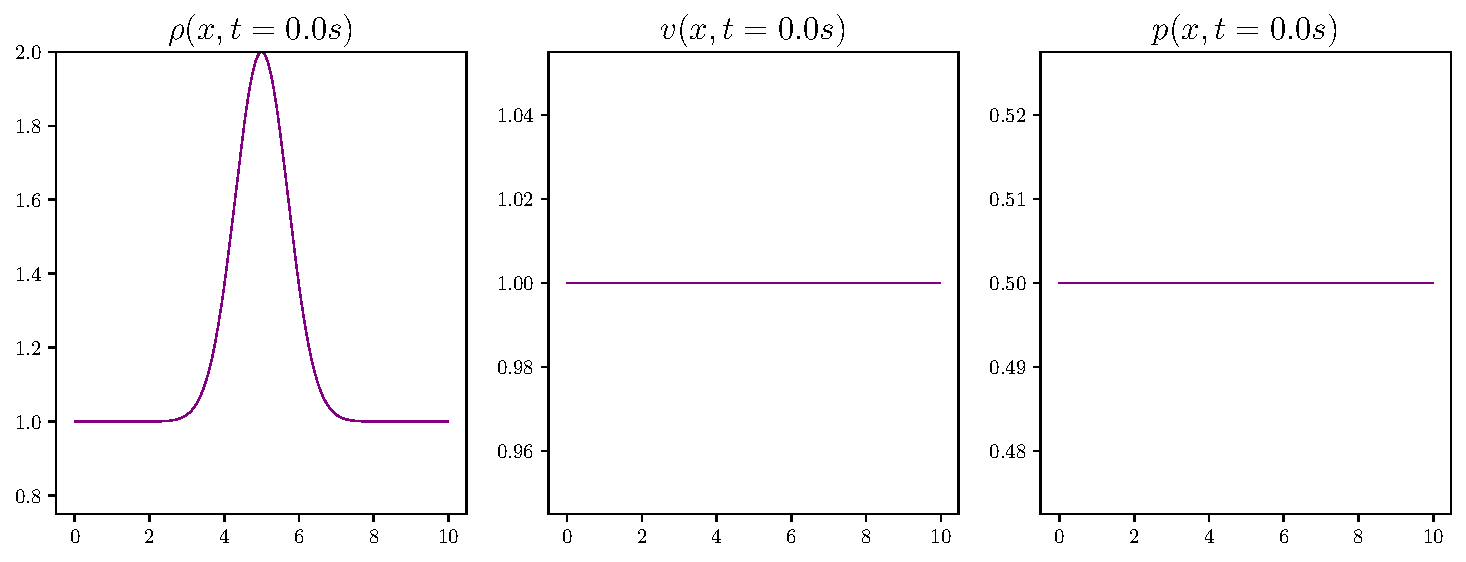
\includegraphics[width=1\linewidth]{../euler1D/plots_en_TDG/set1/graficas/1.pdf}
	\caption{Gráficas para $t=0.0\unit{\s}$}
\end{figure}
\begin{figure}[ht]
	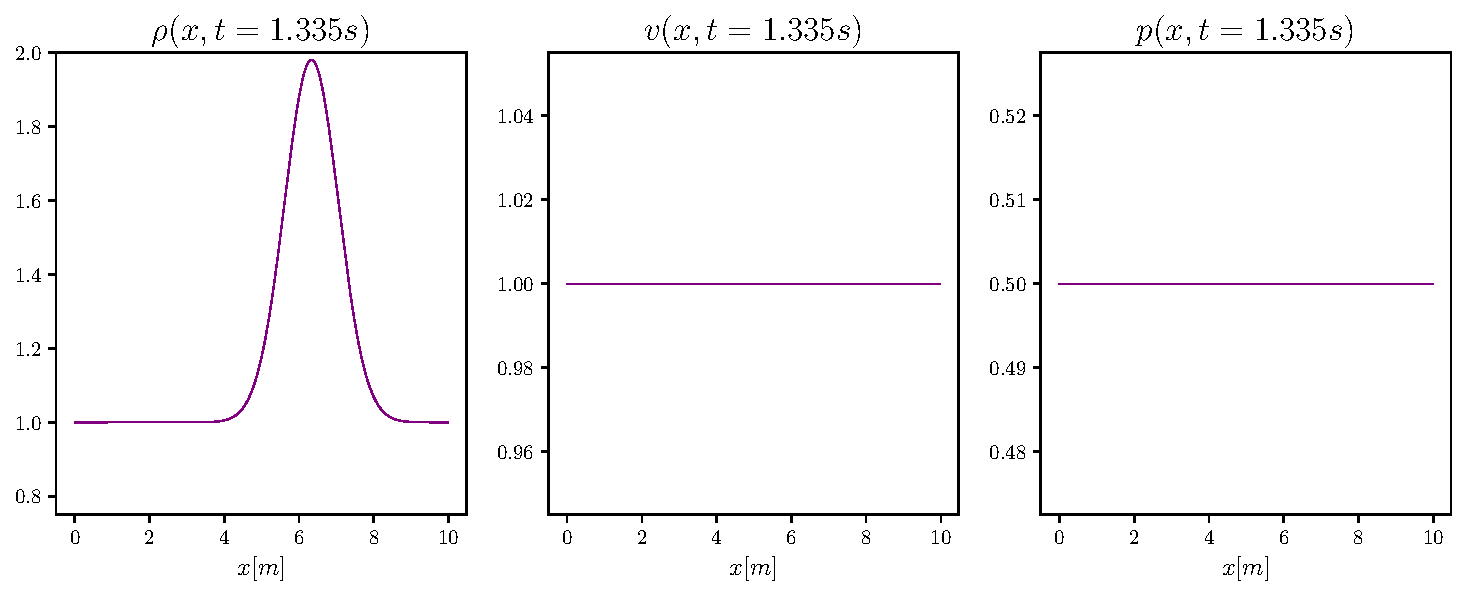
\includegraphics[width=1\linewidth]{../euler1D/plots_en_TDG/set1/135.pdf}
	\caption{Gráficas para $t=1.335\unit{\s}$}
\end{figure}\vspace{\baselineskip}
\begin{figure}[ht]
	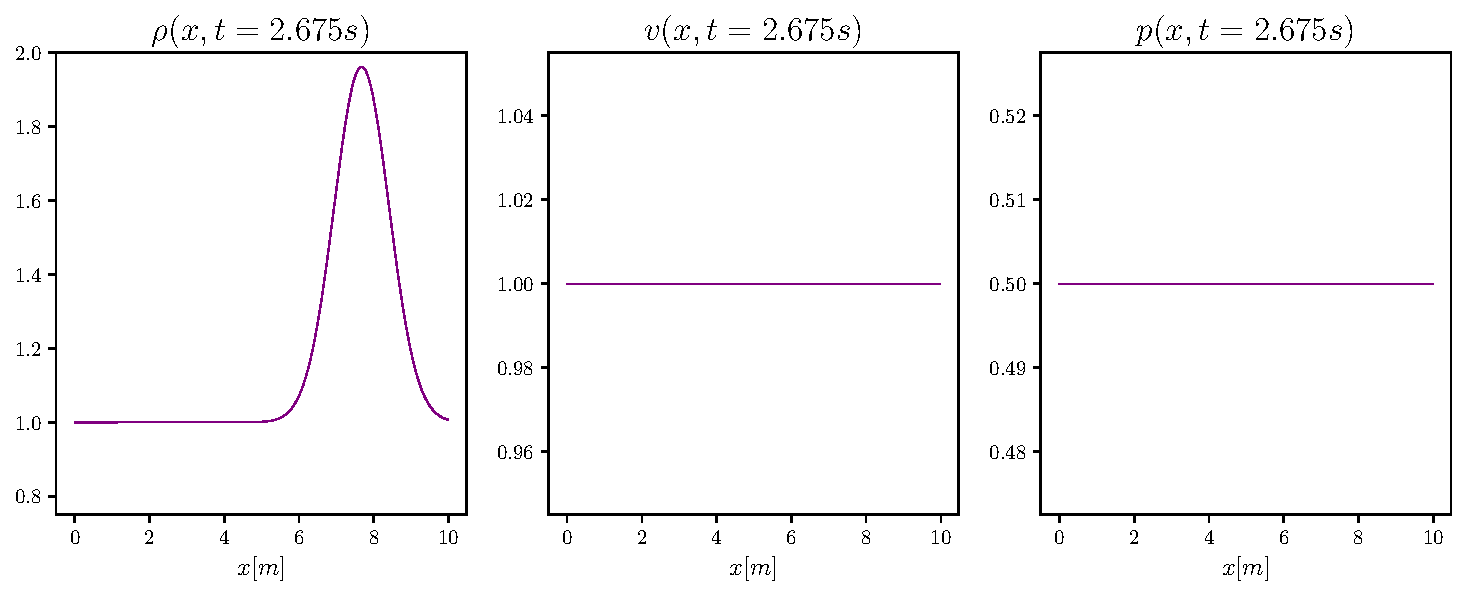
\includegraphics[width=1\linewidth]{../euler1D/plots_en_TDG/set1/269.pdf}
	\caption{Gráficas para $t=2.675\unit{\s}$}
\end{figure}\vspace{\baselineskip}
\begin{figure}[ht]
	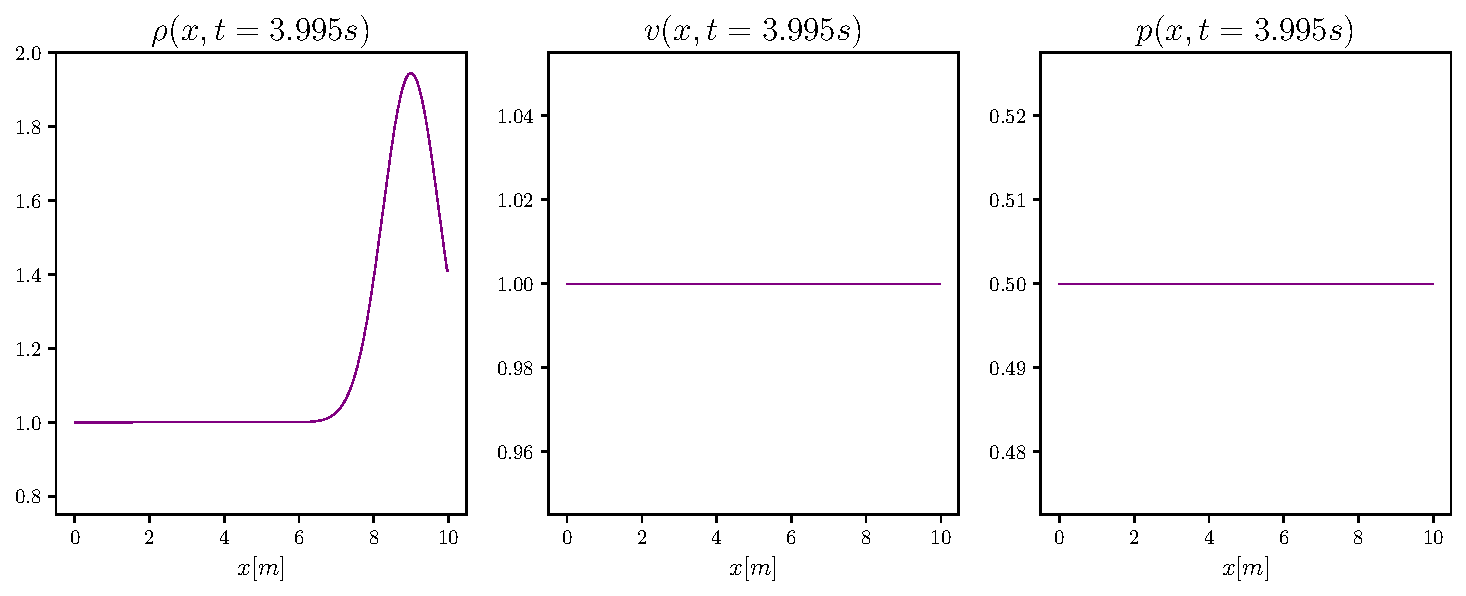
\includegraphics[width=1\linewidth]{../euler1D/plots_en_TDG/set1/401.pdf}
	\caption{Gráficas para $t=3.995\unit{\s}$}
\end{figure}
\subsubsection{Discusión}
Es apreciable el comportamiento de advección que sufre el perfil gaussiano de la densidad del gas. En el instante $t=0.0\unit{\s}$ el centro de la curva gaussiana se encuentra en $x=5\unit{\meter}$, mientras que en el instante $t=3.995\unit{\s}$ éste se encuentra aproximadamente en $x=9\unit{\meter}$. Esta última observación coincide con lo esperado, dado que la velocidad del gas es $1.0\unit{\meter\per\s}$ y es constante a lo largo de toda la simulación.
Por otro lado, destaca que el máximo de la función de densidad no se mantiene constante, sino que se reduce. Esto se debe al error numérico de integración del esquema utilizado.

Esta simulación se realizó sin la corrección de entropía del esquema de Roe ya que no presentó ninguna diferencia cuando se aplicaba la corrección.

\subsection{Simulación con el segundo conjunto de condiciones iniciales}
\label{sec:resultados-set-2}
Las gráficas de las figuras \ref{fig:set2-1} - \ref{fig:set2-4} corresponden a la simulación realizada con las condiciones iniciales descritas en la sección \ref{sec:sod_con_entropy148}. Este conjunto de condiciones se caracteriza por la diferencia entre las magnitudes de las mitades del dominio. La densidad del lado izquierdo triplica la del lado derecho, al igual que sucede con la presión, mientras que la velocidad inicial del fluido es nula. Entonces este sistema puede ser interpretado como la súbita fusión de dos gases con densidad y presión distinta, o en otras palabras, como un \textbf{choque}.
\subsubsection{Gráficas}
\begin{figure}[ht]
	\centering
	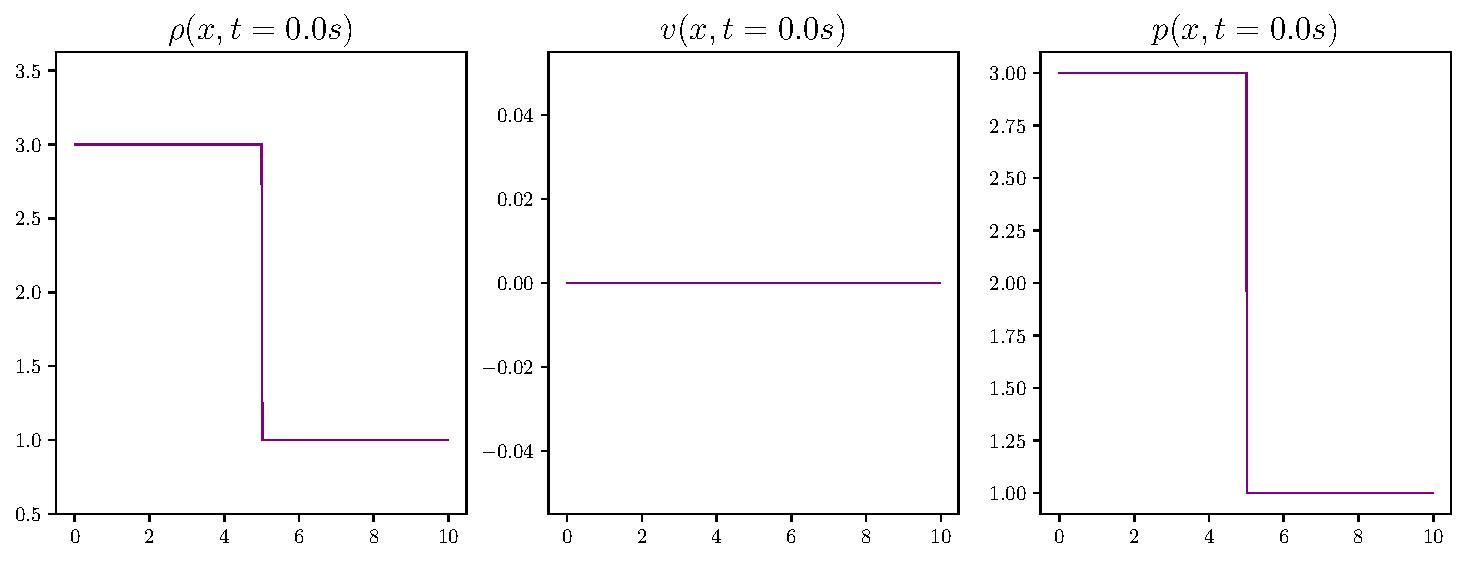
\includegraphics[width=1\linewidth]{../euler1D/plots_en_TDG/set2/1.pdf}
	\caption{Gráficas para $t=0.0\unit{\s}$}
	\label{fig:set2-1}
\end{figure}
\begin{figure}[ht]
	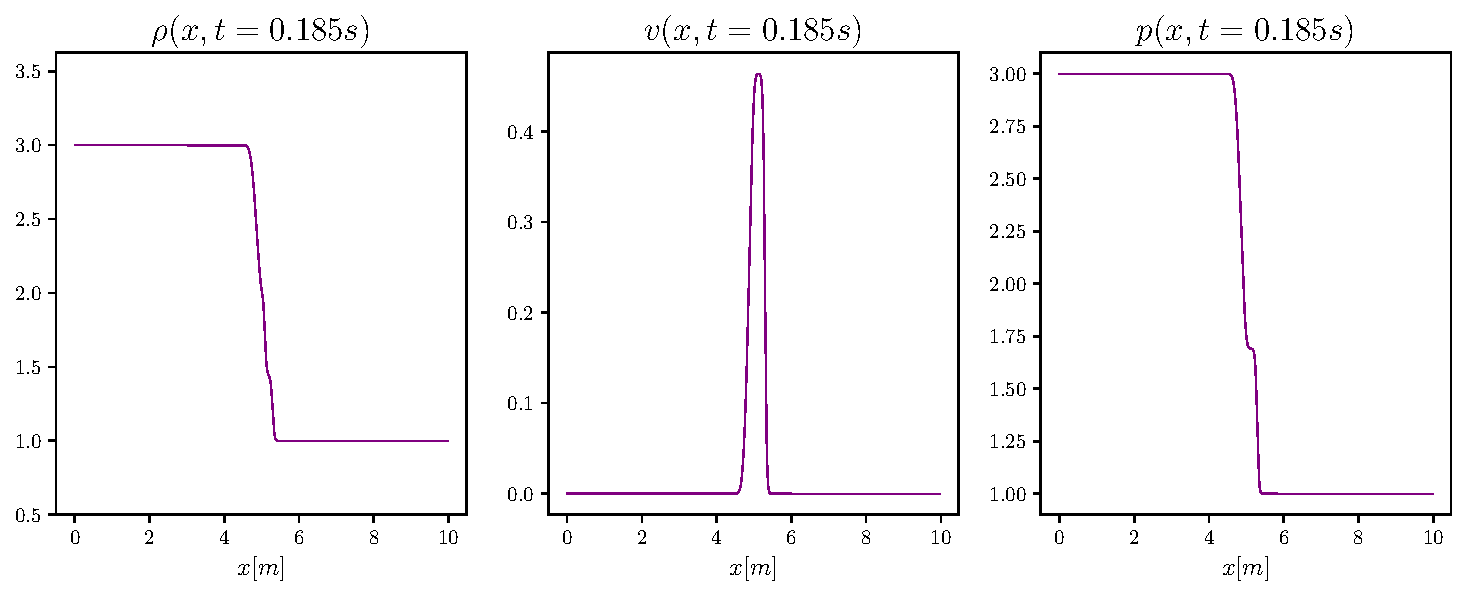
\includegraphics[width=1\linewidth]{../euler1D/plots_en_TDG/set2/20.pdf}
	\caption{Gráficas para $t=0.185\unit{\s}$}
	\label{fig:set2-2}
\end{figure}
\begin{figure}[ht]
	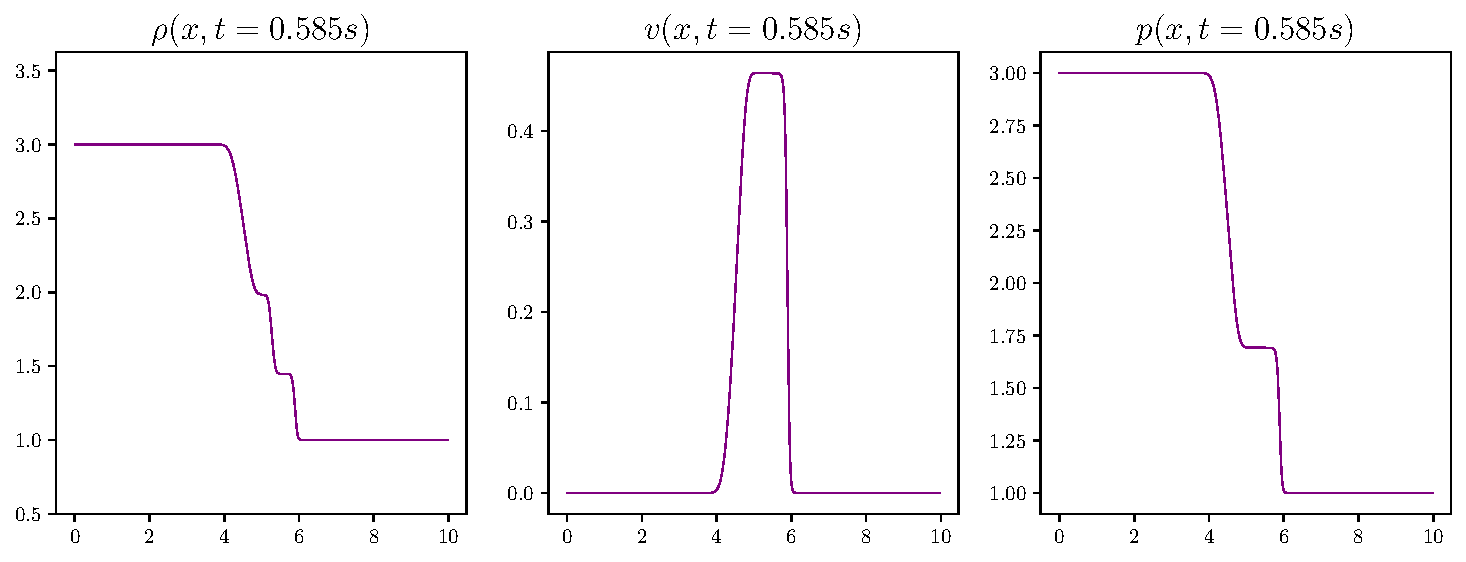
\includegraphics[width=1\linewidth]{../euler1D/plots_en_TDG/set2/60.pdf}
	\caption{Gráficas para $t=0.585\unit{\s}$}
	\label{fig:set2-3}
\end{figure}
\begin{figure}[ht]
	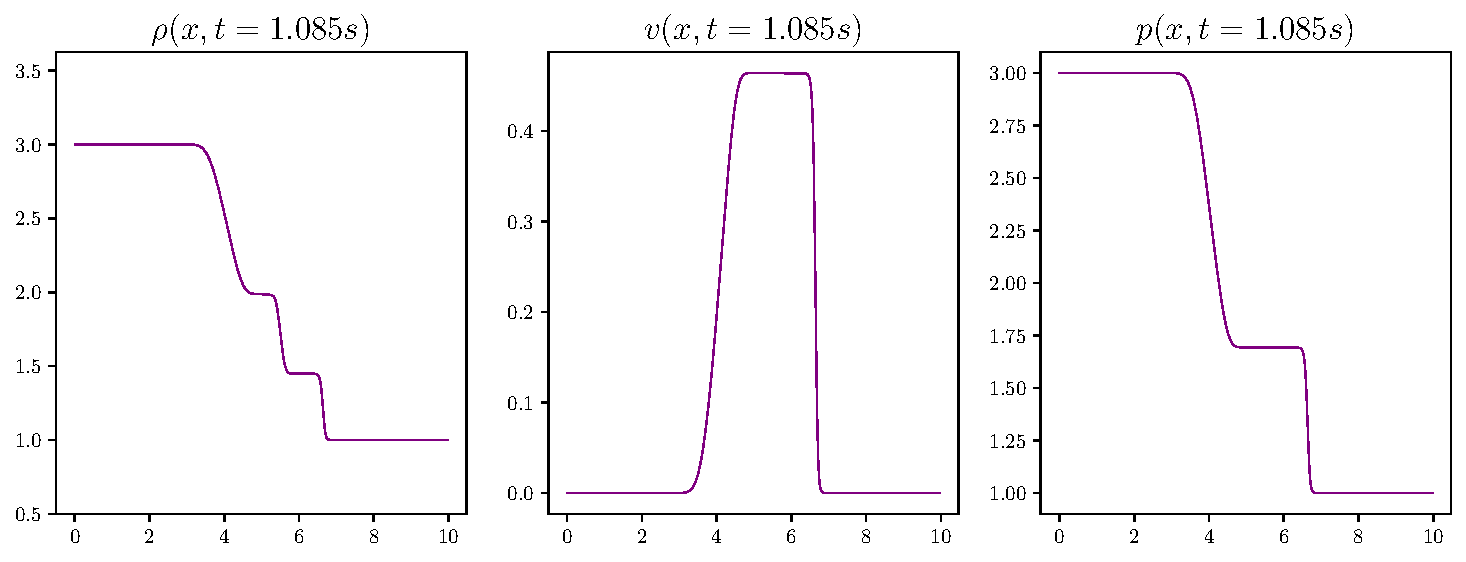
\includegraphics[width=1\linewidth]{../euler1D/plots_en_TDG/set2/110.pdf}
	\caption{Gráficas para $t=1.085\unit{\s}$}
	\label{fig:set2-4}
\end{figure}
\subsubsection{Discusión}
En esta simulación se destaca principalmente la manifestación de ondas de choque y de rarefacción en todas las variables del gas. La densidad se divide en tres ondas; una de choque, que avanza hacia la derecha, y otra de rarefacción, que avanza a la izquierda. La onda intermedia entre las dos últimas se conoce como \textbf{discontinuidad de contacto} \cite{thesis-euler-godunov} y se caracteriza por ser una discontinuidad en la densidad únicamente, ya que la presión y velocidad permanecen constantes. La discontinuidad de contacto también está estrechamente relacionada con la diferencia de temperatura entre las partes del gas que ésta divide \cite{LeVeque}. 

Por otro lado, es notable la eficiencia del esquema de Roe al capturar ondas de choque (discontinuidades) como soluciones.

Esta simulación se realizó sin la corrección de entropía del esquema de Roe ya que no presentó ninguna diferencia cuando se aplicaba la corrección.

\subsection{Simulación con el tercer conjunto de condiciones iniciales}
Se experimentó con el conjunto de condiciones iniciales descrito en la sección \ref{sec:leveque_sin_entropy714}. Este conjunto es similar al discutido anteriormente, con la diferencia que la velocidad inicial de este conjunto no es nula, sino que tiene un valor constante en todo el dominio. Este problema surge a partir de una forma de evaluar la aparición de ondas de rarefacción sónica, de tal manera que pone a prueba la función de corrección de entropía utilizada.

\subsubsection{Gráficas de la simulación sin corrección de entropía}
\begin{figure}[ht]
	\centering
	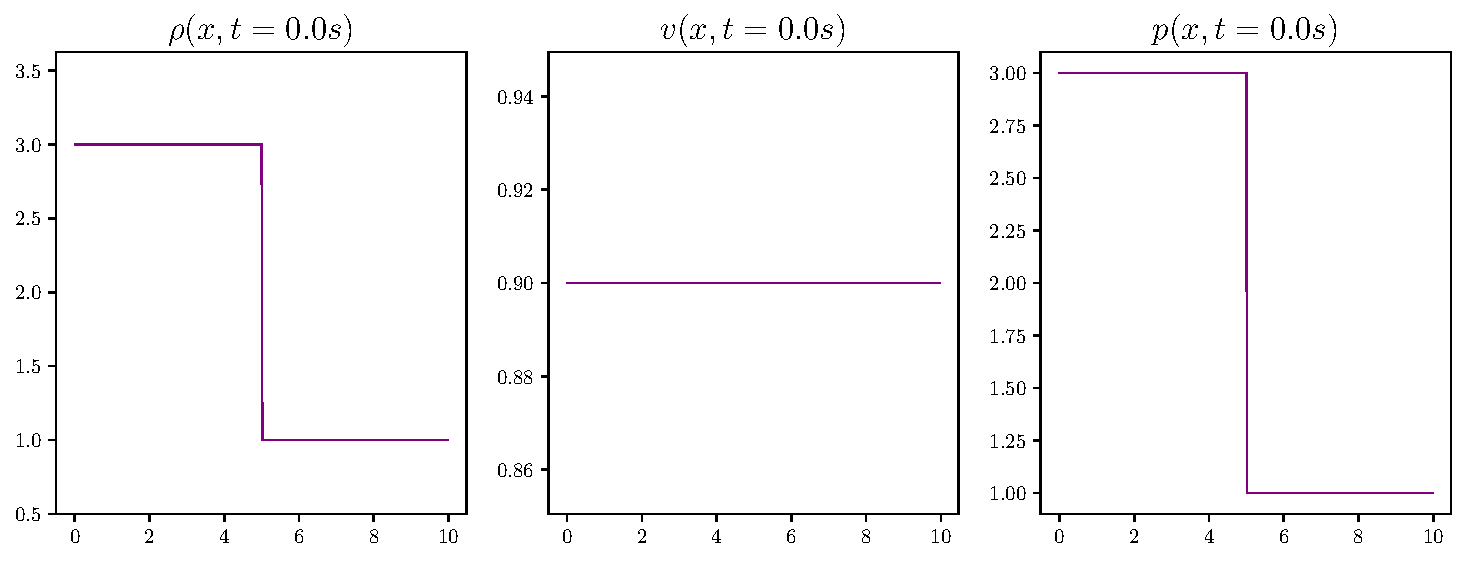
\includegraphics[width=1\linewidth]{../euler1D/plots_en_TDG/set3/leveque_sin_entropy714/1.pdf}
	\caption{Gráficas para $t=0.0\unit{\s}$}
\end{figure}
\begin{figure}[ht]
	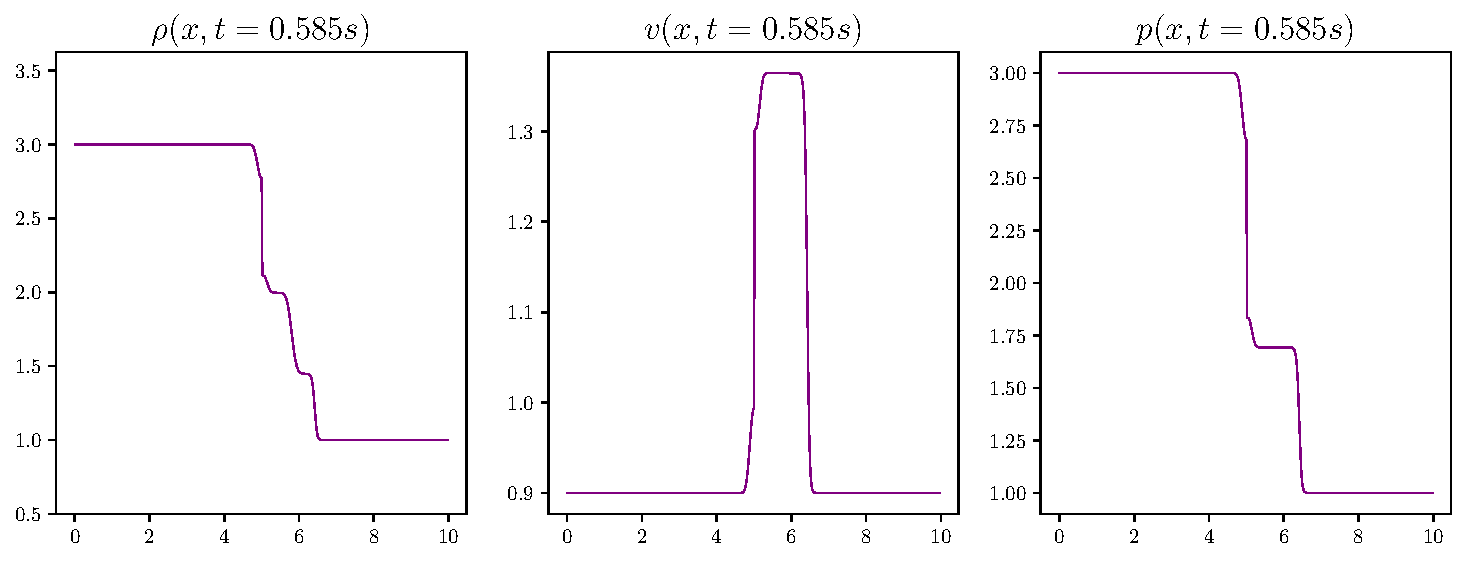
\includegraphics[width=1\linewidth]{../euler1D/plots_en_TDG/set3/leveque_sin_entropy714/60.pdf}
	\caption{Gráficas para $t=0.585\unit{\s}$}
\end{figure}
\begin{figure}[ht]
	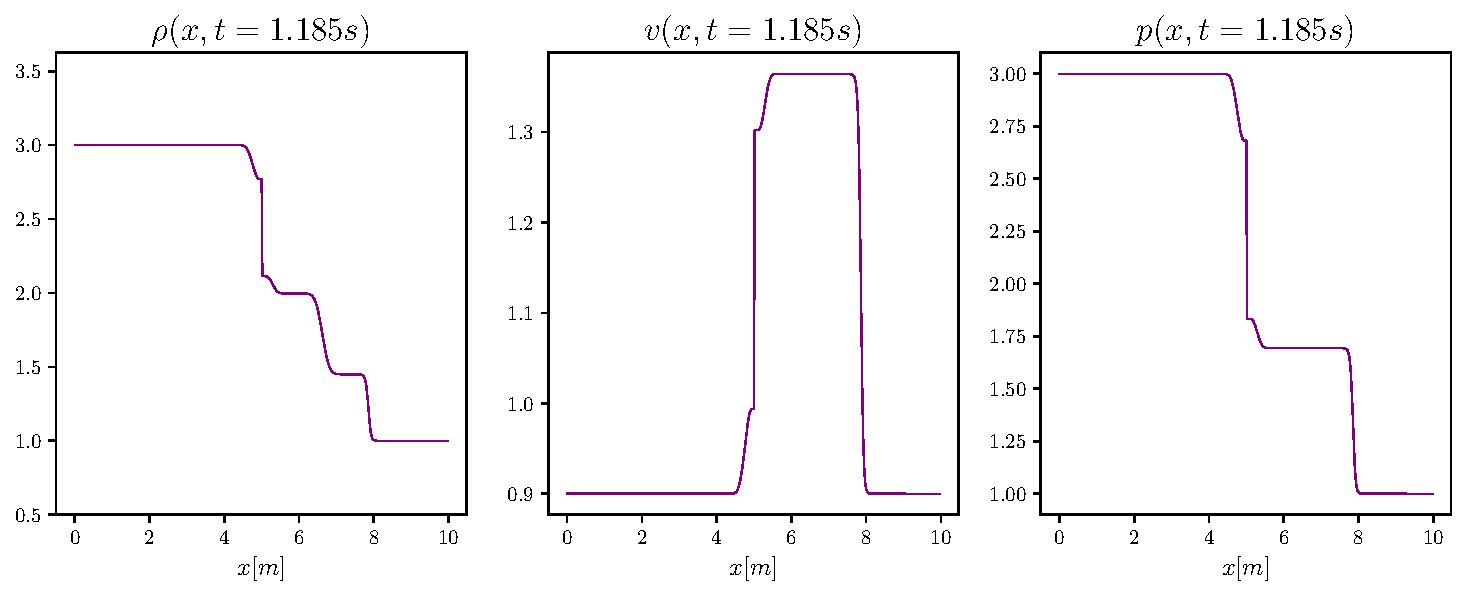
\includegraphics[width=1\linewidth]{../euler1D/plots_en_TDG/set3/leveque_sin_entropy714/120.pdf}
	\caption{Gráficas para $t=1.185\unit{\s}$}
\end{figure}
\clearpage

\subsubsection{Gráficas de la simulación con corrección de entropía}
\begin{figure}[ht]
	\centering
	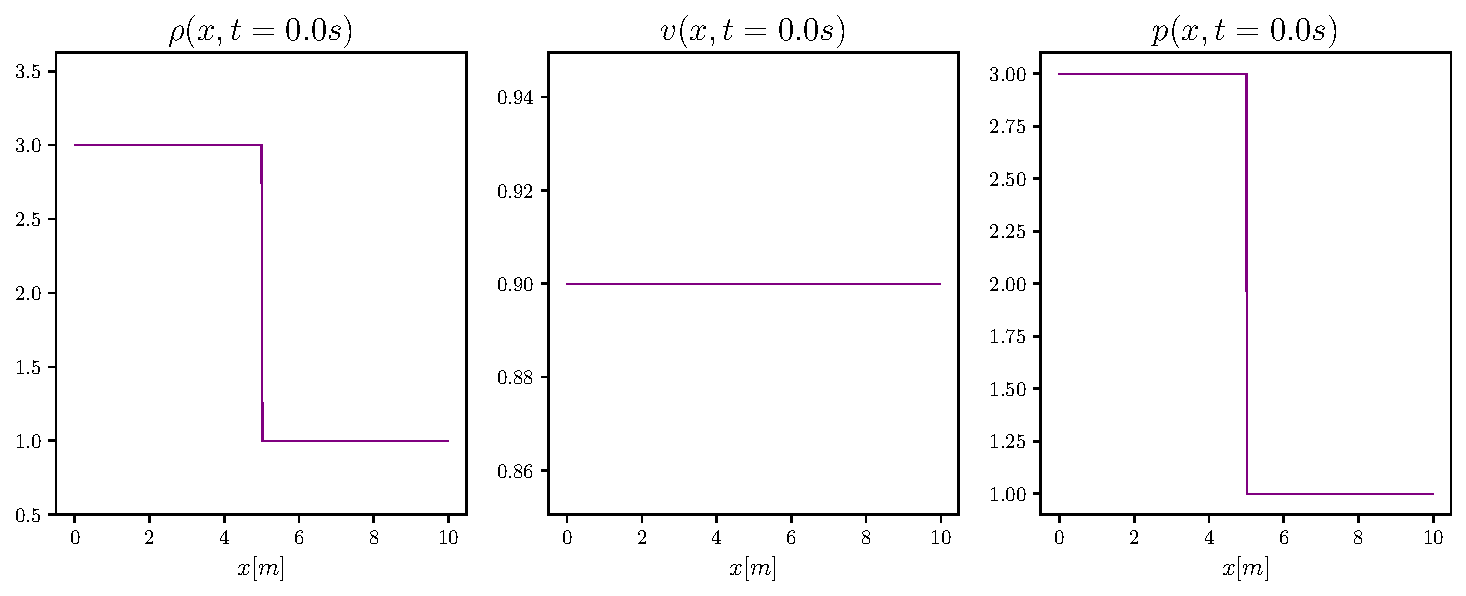
\includegraphics[width=1\linewidth]{../euler1D/plots_en_TDG/set3/leveque_con_entropy123/1.pdf}
	\caption{Gráficas para $t=0.0\unit{\s}$}
\end{figure}
\begin{figure}[ht]
	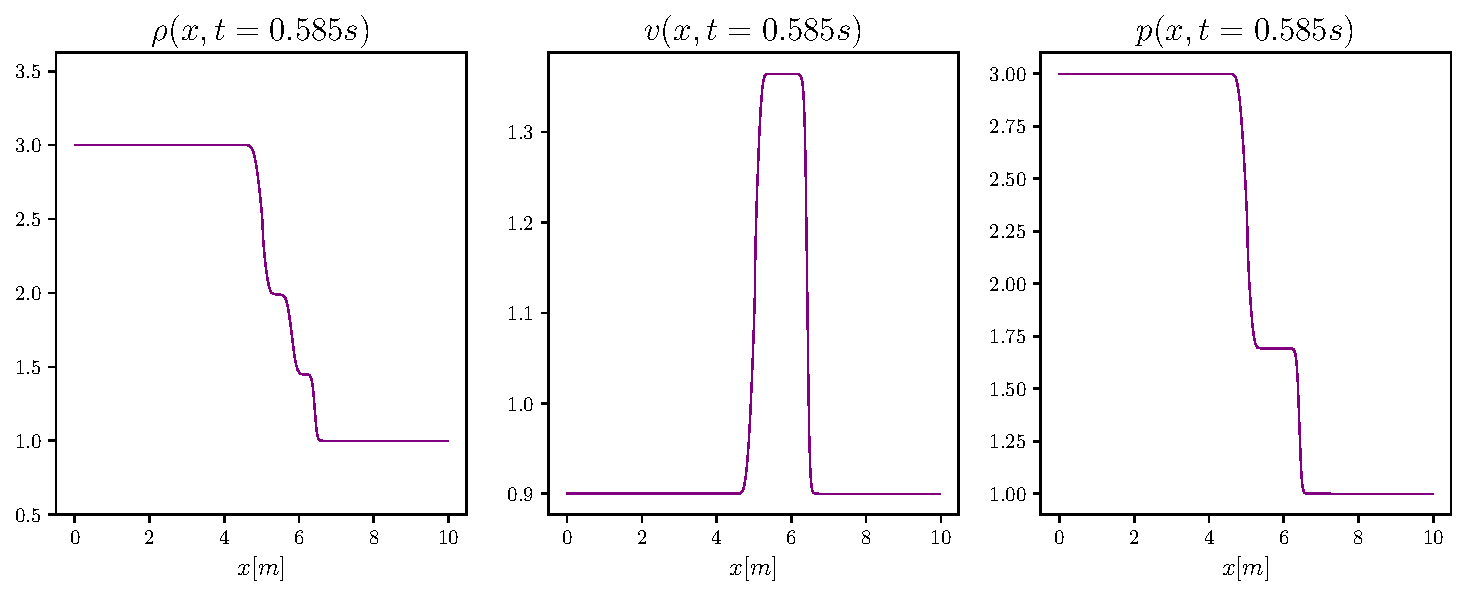
\includegraphics[width=1\linewidth]{../euler1D/plots_en_TDG/set3/leveque_con_entropy123/60.pdf}
	\caption{Gráficas para $t=0.585\unit{\s}$}
\end{figure}
\begin{figure}[ht]
	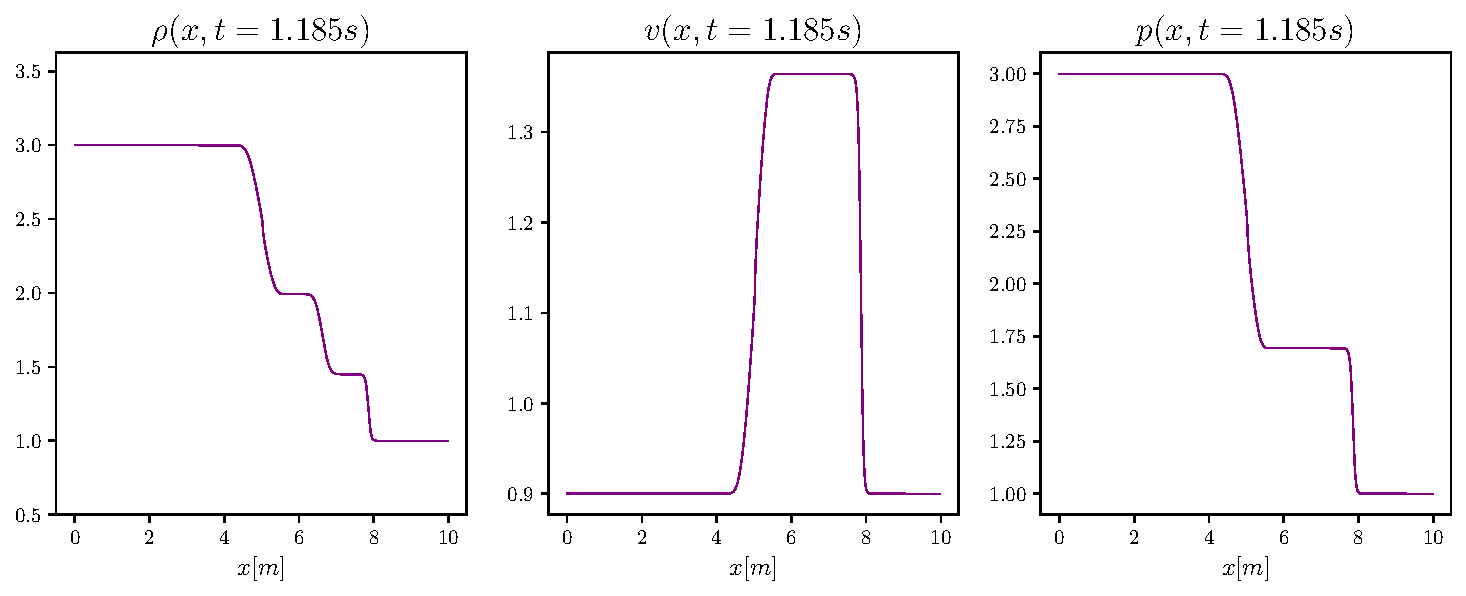
\includegraphics[width=1\linewidth]{../euler1D/plots_en_TDG/set3/leveque_con_entropy123/120.pdf}
	\caption{Gráficas para $t=1.185\unit{\s}$}
	\label{fig:ultima-sin-entropy}
\end{figure}\vspace{5cm}

\subsubsection{Discusión}
Se puede notar la similitud entre los resultados de esta simulación y la correspondiente al segundo conjunto. Sin embargo, en este caso el programa sin la condición de entropía no logra capturar las ondas de rarefacción, como puede notarse en la figura \ref{fig:ultima-sin-entropy}; notando que especialmente la onda de rarefacción que avanza a la izquierda (identificada en los resultados de la sección anterior) aparece dividida por una discontinuidad. En cambio, los resultados producidos al utilizar la corrección de entropía sí son consistentes con las ondas de rarefacción esperadas; se puede notar la similitud entre estos resultados y los de la sección \ref{sec:resultados-set-2}. La onda de rarefacción izquierda no presenta discontinuidades en estos resultados.